\subsection{Number turns in a time t}
In order to continue the exploration of the combination of minimax and MCTS started in the previous section,
a histogram was made to compare the number of turns in a certain time for minimax and MCTS. This histogram can
be found on the figure~\ref{fig:histo}.\\

The graph presented earlier gives you an idea of what the histogram will look like. Indeed, the minimax rounds always take less time than those made by MCTS.
The time taken per minimax is always between 1 and 3 seconds. By the way, on the histogram, some times look negative but this is simply the distribution chosen for the buckets used.
The minimax algorithm is much more stable than MCTS, the times are concentrated in the first two buckets of the histogram. For MCTS, the time taken for the rounds changes a lot.
A peak is reached between 7 and 9 seconds, i.e. more than 3 times the average time for minimax.

However, the number of laps that take more than 15 seconds is quite low compared to the rest. Even though MCTS takes longer than minimax,
this time is still reasonable and considering that this algorithm may be more efficient at the beginning of a game, it would certainly be advantageous to use both algorithms.

\begin{figure}[ht]
    \centering
    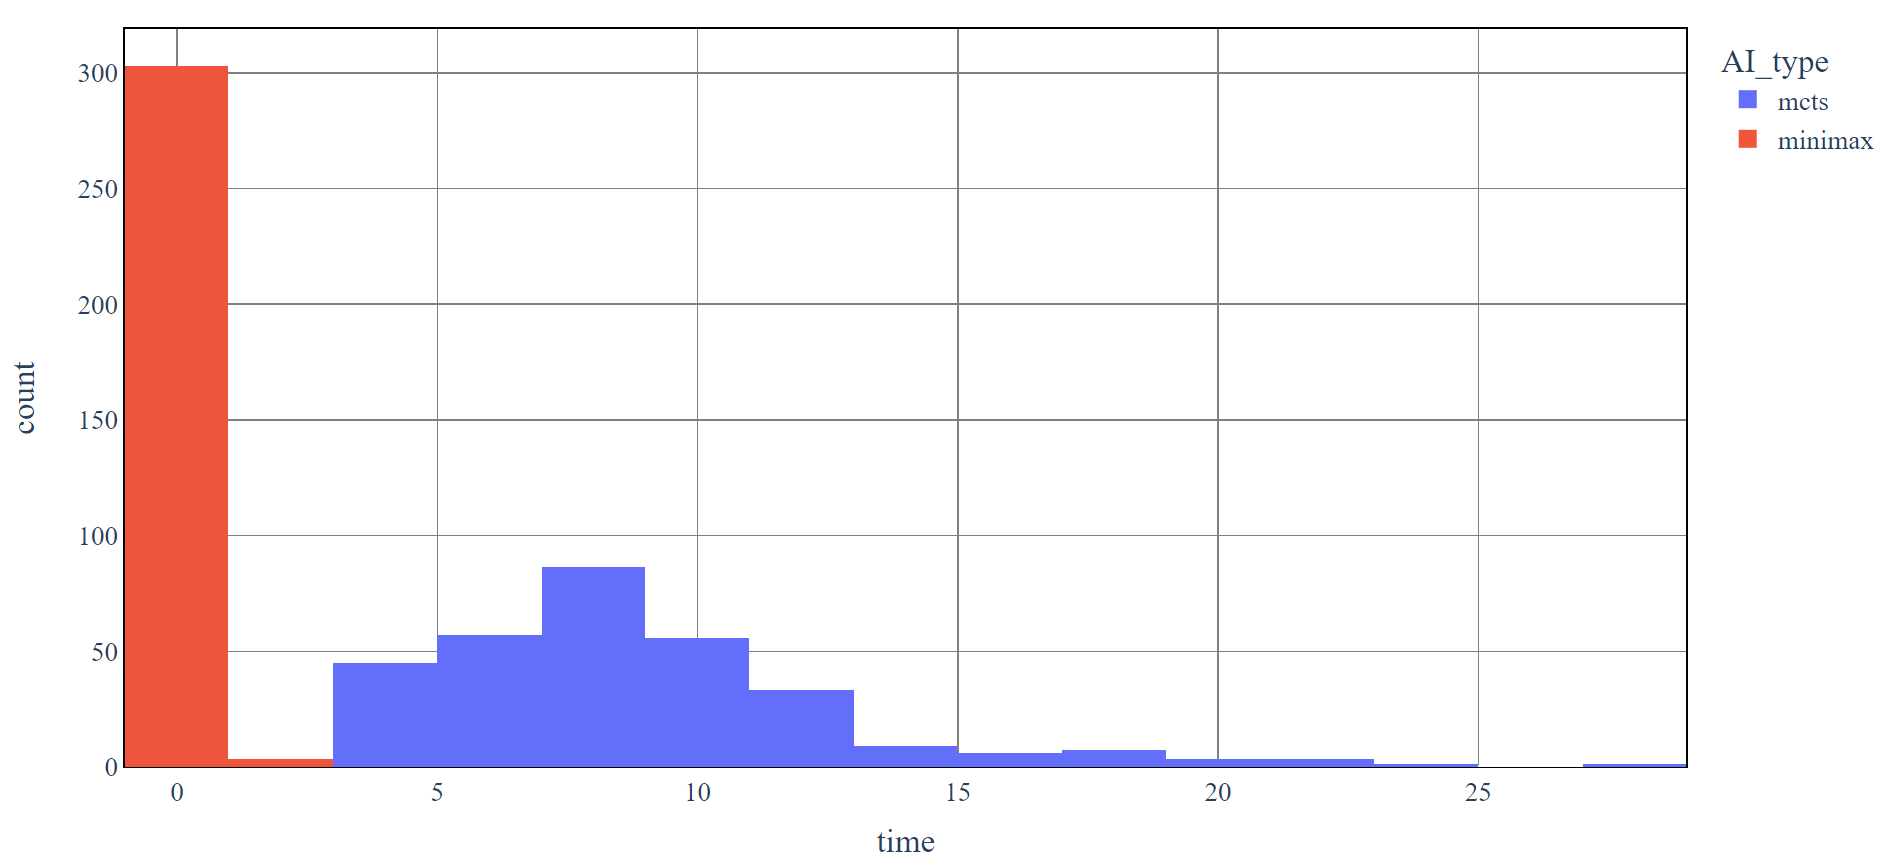
\includegraphics[width=\linewidth]{nb_turn_in_time_t.png}
    \caption{Histogram of number of turns of both used algorithms that take a certain time [s].}
    \label{fig:histo}
\end{figure}